% Provide commands to typeset proof trees in the style of sequent calculus and related systems
\usepackage{ebproof}

% https://tex.stackexchange.com/a/32103
% https://ctan.org/pkg/amscd
\usepackage{amsmath, amsthm, amscd}
\newtheorem*{claim}{Claim}

% Extending the array and tabular environments
% FTR the modern approach for document writers seems to be to use package nicematrix or package tabularray instead of package array.
\usepackage{tabularray}

% Control layout of itemize, enumerate, description
\usepackage{enumitem}

\usepackage{tikz}
\usetikzlibrary{arrows,positioning,trees,decorations.pathmorphing,shapes}
\definecolor{Maroon}{rgb}{0.45,0.025,0.05}

\usepackage{graphicx}
\graphicspath{ {./images/} }

\usepackage{pdfpages}

\usepackage[british]{babel} % or https://ctan.org/pkg/polyglossia

% Alegreya fonts
\usepackage[oldstyle]{Alegreya}
% Euler-Math provides all AMS symbols
\usepackage{euler-math}
\renewcommand\qedsymbol{$\QED$}
% St Mary Road symbols for theoretical computer science
\usepackage{stmaryrd}

\usepackage{geometry}
\geometry{left=2cm, right=2cm, top=2cm, bottom=2cm, includehead, includefoot}

\usepackage[onehalfspacing]{setspace}
\usepackage[skip=0.75\baselineskip plus 2pt]{parskip}

\usepackage{fancyhdr}
\pagestyle{fancy}
\fancyhead[L]{Matriculation Number: 230030434}
\fancyhead[R]{\thepage}
\fancyfoot[C]{}
\setlength{\headheight}{14.5pt}

\usepackage{hyperref}  % Loading hyperref last: very few packages should come later than this one
\hypersetup{
   colorlinks = true,  % to avoid the borders around hyperlinks
   citecolor  = black,
   filecolor  = black,
   linkcolor  = black,
   urlcolor   = black,
}

% These definitions are for shorthands that might come in handy
\def\pair #1{\langle{#1}\rangle}
\def\diam{\lozenge}
\def\bx{\Box}
%% Y-right argument separator symbol
\DeclareSymbolFont{stmry}{U}{stmry}{m}{n}
\DeclareMathSymbol{\Yright}{\mathbin}{stmry}{"07}
%% Labels for rules for natural deduction proofs
\NewDocumentCommand{\ci}{m}{\ensuremath{{\to}I^{#1}}}
\NewDocumentCommand{\ce}{}{\ensuremath{{\to}E}}
\NewDocumentCommand{\ai}{}{\ensuremath{{\land}I}}
\RenewDocumentCommand{\ae}{}{\ensuremath{{\land}E}}
\NewDocumentCommand{\di}{}{\ensuremath{{\lor}I}}
\NewDocumentCommand{\de}{m}{\ensuremath{{\lor}E^{#1}}}
\NewDocumentCommand{\negi}{m}{\ensuremath{{\lnot}I^{#1}}}
\NewDocumentCommand{\nege}{}{\ensuremath{{\lnot}E}}
\NewDocumentCommand{\bote}{}{\ensuremath{{\bot}E}}
\NewDocumentCommand{\dne}{}{\ensuremath{DNE}}
\NewDocumentCommand{\bi}{m}{\ensuremath{{\leftrightarrow}I^{#1}}}
\NewDocumentCommand{\be}{}{\ensuremath{{\leftrightarrow}E}}
\NewDocumentCommand{\boxe}{}{\ensuremath{\bx E}}
\NewDocumentCommand{\boxi}{}{\ensuremath{\bx I}}
\NewDocumentCommand{\diame}{m}{\ensuremath{\diam E^{#1}}}
\NewDocumentCommand{\diami}{}{\ensuremath{\diam I}}
\NewDocumentCommand{\une}{}{\ensuremath{\forall E}}
\NewDocumentCommand{\uni}{}{\ensuremath{\forall I}}
\NewDocumentCommand{\exe}{m}{\ensuremath{\exists E^{#1}}}
\NewDocumentCommand{\exi}{}{\ensuremath{\exists I}}

\ExplSyntaxOn
\NewDocumentCommand { \generate } { m m }
  {
    \str_new:N \l_type
    \str_new:N \l_idx

    \str_set:Nn \l_type {#1}
    \str_set:Nn \l_idx  {#2}

    \str_if_eq:VnTF \l_type {proj}
      {
        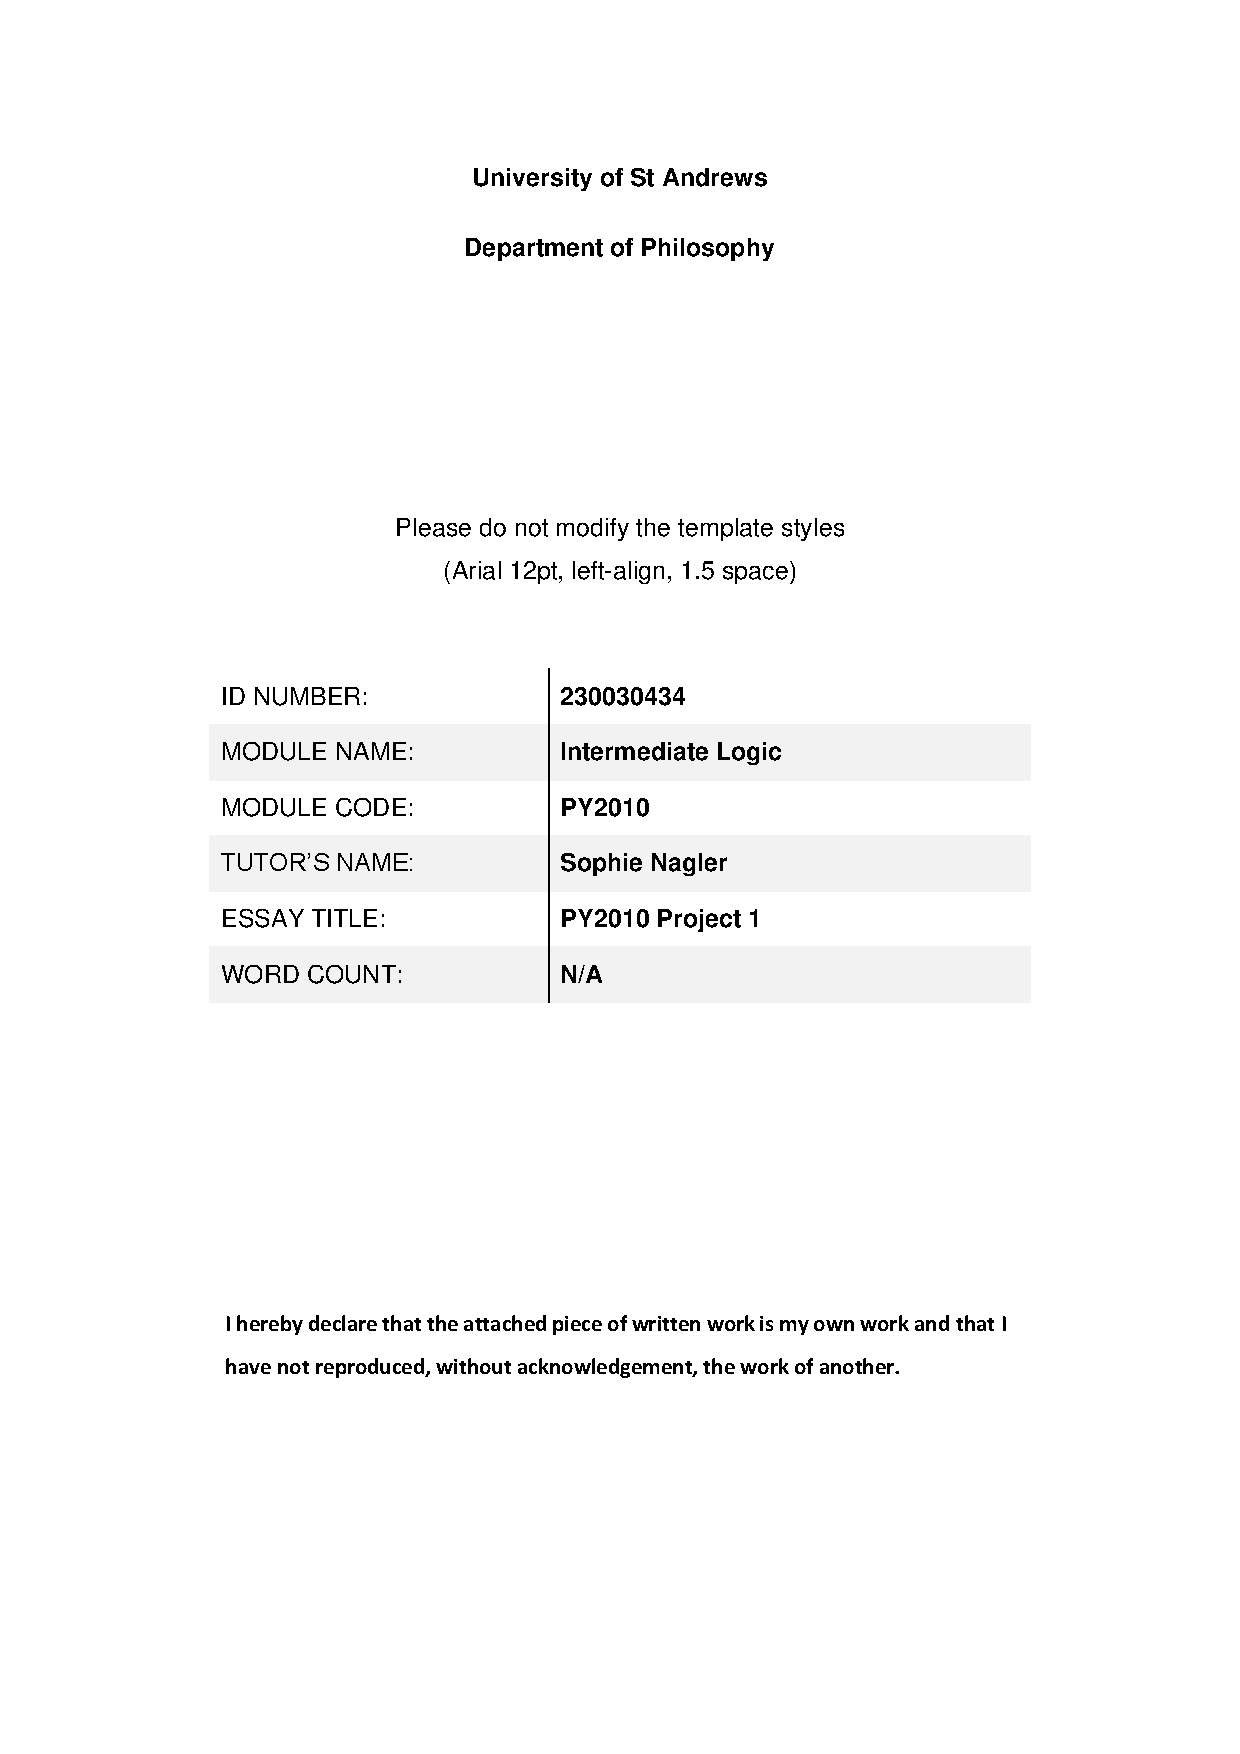
\includepdf[pages=-]{\l_type\l_idx/cover}
        \setcounter{page}{1} % FIXME: https://stackoverflow.com/questions/501378/how-can-i-start-pagenumbers-where-the-first-section-occurs-in-latex

        \foreach \i in {1, 2, ..., 5}
          {
            \IfFileExists {\l_type\l_idx/\i}
              { \input {\l_type\l_idx/\i} \newpage }
          }
      }
      {
        % \thispagestyle{empty}
        % \begin{tikzpicture}[remember picture,overlay]
        % \node[anchor=north east, yshift=-22pt, xshift=-36pt]%
        %     at (current page.north east)
        %     {\includegraphics[width=0.37\textwidth]{crest}};
        % \end{tikzpicture}

        \begingroup
          \centering
          \huge \textsc{py2010}~Intermediate~Logic \\
          \large taught~by~Prof~Greg~Restall \\ [0.4em]
          \LARGE Week~\uppercase\expandafter{\romannumeral\l_idx}~Exercises \\ [0.4em]
          \large \today \\ [0.6em]
          \begin{spacing}{1}
          \parbox{0.53\textwidth} 
            { \normalsize
              I~ hereby~ declare~ that~ the~ attached~ piece~ of~ written~ work~ is~ my~ own~ work~ and~ that~ I~ have~ not~ reproduced,~ without~ acknowledgement,~ the~ work~ of~ another.
            } \\
          \end{spacing}
        \endgroup

        \foreach \i in {1, 2, ..., 6}
          {
            \IfFileExists {\l_type\l_idx/\i}
              {
                \section*{Exercise~\i}
                \input {\l_type\l_idx/\i}
              }
          }
      }
  }
\ExplSyntaxOff
